% Copyright (c) 2005-2009 Center for Urban Simulation and Policy Analysis,
% University of Washington.  Permission is granted to copy, distribute and/or
% modify this document under the terms of the GNU Free Documentation License,
% Version 1.2 or any later version published by the Free Software Foundation;
% with no Invariant Sections, no Front-Cover Texts, and no Back-Cover Texts.
% A copy of the license is included in the section entitled "GNU Free
% Documentation License".

\chapter{Installation}
\label{appendix:installation}

\index{installating Opus}

\section{Installing Opus}

Opus has been run and tested on Windows, Linux and Macintosh OS X\@.  (It
should also run on any other platform that Python and its libaries run on,
but we've not tested others.)  Instructions for installing Opus, and
UrbanSim, which is bundled with it, are kept online at
\url{http://www.urbansim.org/download/}.  There is also a copy of the
instructions in the source code tree --- open the file 
\file{opus_docs/installation/index.html} in a web browser.

We provide both \emph{stable releases} and \emph{development versions} of
Opus/UrbanSim.  Each stable release has a unique version number, such as
4.1.2 (see Appendix \ref{appendix:version-numbers}).
Generally, we recommend using the latest stable release of
Opus/UrbanSim.  The system is under continuing development, and the other
possibility is using the latest development version from our source code
repository (not always recommended for the faint-of-heart).

\subsection{Windows Installer}

For users with a computer running Windows, we currently recommend
installing the latest development version using the Windows Installer,
which is downloadable from
\url{http://www.urbansim.org/opus/installer/opus_installer.exe}.  Step by
step details for using the installer are available at
\url{http://www.urbansim.org/docs/installation}.  Follow these instructions
on the web for the installation, and return to this document afterward for
recommendations for testing your installation (Section
\ref{appendix:testing-your-installation}).  The installer launches other
installers for supporting packages during the install process, so you need
to be connected to the Internet for the installer to download files during
the installation.  Please be patient --- the installation takes 20-30
minutes depending on your connection speed.

\subsection{Installing on Other Platforms}

Step by step instructions for installing on other platforms (as well as on
windows by hand rather than with the installer) are available at
\url{http://www.urbansim.org/docs/installation}.  First select either the
latest stable release or the latest development version, and then the web
page for your particular platform.

\subsection{Testing Your Installation}
\label{appendix:testing-your-installation}

Once Opus is installed, it is a good idea to test whether it is installed
correctly.  The installation involves downloading and installing numerous
components (all managed by the Windows installer, if you're using that).
There are times when a component does not download properly and fails to
install, and particularly when using the Windows installer you might not
notice this.  Here are a few simple tests to check whether Python and the
key libraries are properly installed.

\begin{enumerate}
\item Start a command window or shell.  On Windows, this can be done from
  the start menu \verb#run# and entering \verb#cmd#.
\item Type \verb#python# and press Enter (for brevity, I will not repeat
  the press Enter at the end of each command - it is implied).  A Python
  prompt should appear, as \verb#>>>#.
\item Type \verb#import numpy#.  It should just generate another Python
  prompt, which means it successfully imported the Numpy library.  If it
  fails, you will see an errror, and need to exit Python and reinstall
  Numpy.  To see what version of Numpy is installed, type
  \verb#numpy.__version__#.
\item Repeat the import step with the following libraries: scipy,
  matplotlib, sqlalchemy, and PyQt4 (the capitalization matters).  If all
  of these import without reporting an error, the main libraries are
  installed correctly.  The version number for sqlalchemy should be at
  least 0.4.3 at the time of this writing.
\item Finally, type \verb#import opus_core#.  This verifies that the
  \package{opus_core} package has been downloaded and that Python can find
  it.  (If it can find \package{opus_core}, it can probably find the others
  \ldots) 
\end{enumerate}

To exit an interactive Python session, type \kbd{quit()}.  (As a shortcut
for exiting Python, you can instead type control-z on windows, or control-d
on Macintosh or linux.)

\subsection{Updating the Software}

The software is being continuously developed and refined, with bug fixes
and new features being added.  In order to get these updates, or to
download and install other Opus Packages not initially installed, users
will need an application that can retrieve updates and packages from the
Subversion repository for the software.  Subversion is a version control
system used by many software development projects, and there are many free
software tools available for accessing it.  One of these, on the Windows
platform, is Tortoisesvn, available from \url{http://tortoisesvn.tigris.org/}.
Users can download and install this package, and it will extend the Windows
Explorer file browser, allowing packages to be \emph{checked out} of the
repository (downloaded for the first time), or \emph{updated} if they have
already been checked out previously.  Subversion compares the version on
your local machine with the version on the server, and if there is a newer
version of any component, it will download it and replace the version on
your machine with the most current one available.

To check out (download for the first time) any package from the Opus
repository, if you have installed Tortoisesvn, right-click on the opus/src
folder in the Windows Explorer, and the menu will contain new entries for
interacting with Subversion.  Select the \verb#SVN Checkout# option.  For a
stable release, say version 4.2.0, use the url
\url{https://trondheim.cs.washington.edu/svn/opus/tags/4.2.0}, plus the
name of any package you wish to check out.  For a package from the latest
development version use the url
\url{https://trondheim.cs.washington.edu/svn/opus/trunk}, plus the name of
any package you wish to check out.  The target local directory should be
under the Opus\_HOME/src directory, and take the same name as the Opus
Package you are checking out.  An example of this checkout dialog is shown
in Figure \ref{fig:tortoisesvn}.  There are other Subversion clients
available for Windows, OS X and Linux, and any of them should work
equivalently well for obtaining Opus packages.  Eventually, this
functionality may be embedded into the Opus GUI.

\begin{figure}[htp]
\begin{center}
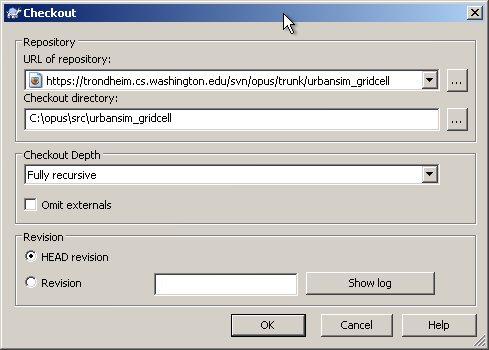
\includegraphics[scale=0.4]{graphics/tortoisesvn.png}
\end{center}
\caption{Checking Out a Package using the TortoiseSVN Subversion Client}
\label{fig:tortoisesvn}
\end{figure}

Once a user makes changes on their local machine to any content that has
been checked out from the repository, the changed file will be inconsistent
with the version in the repository.  In many cases, this is fine, but if
the file is updated by someone else and checked into the repository, then
the next time you update from the repository, you will have conflicting
changes in the file you have modified.  There are tools available to
reconcile the conflicts, but the best approach for most users is to isolate
the places you want to make changes to a location that will not have
collisions with ongoing updates in the repository.  A project\_configs
directory is intended for users to create and manage their own projects.
If the user needs to modify Python modules within the various Opus
packages, these can most easily be handled by creating another Opus package
of your own that \emph{inherits} from the package you want to change, and
contains only the modified versions of files.  Note that Opus packages can
be updated from the repository at any time by selecting the directory (or
all of them at once), right-clicking, and selecting the menu item for
\verb#SVN Update#.

